\documentclass[10pt,conference,compsocconf]{IEEEtran}

%Deadline: April 8, 2015
%Call for papers: http://www.computer.org/web/computingnow/swcfp6

\usepackage{url}
\usepackage[table,xcdraw]{xcolor}
\usepackage{eurosym}
\usepackage{amsfonts}
\usepackage{balance}
\usepackage{cite} %this package is awesome - it reorders lists of citations to be in numeric order
\usepackage[pdftex]{graphicx}
\usepackage{pifont}
\usepackage{eqparbox}
\graphicspath{ {}{img/} }
\DeclareGraphicsExtensions{.pdf,.jpg,.png}

\hyphenation{second-ly ap-pen-dix}

\clubpenalty = 10000
\widowpenalty = 10000
\displaywidowpenalty = 10000

\newcommand{\todo}[1]{\textbf{TODO: #1}}

\begin{document}
%
% paper title
% can use linebreaks \\ within to get better formatting as desired
\title{End-User Refactoring}
%\title{Perspectives on End-User Refactoring: Past, Present, and Future}

\author{\IEEEauthorblockN{Felienne Hermans, David Hoepelman}
\IEEEauthorblockA{Delft University of Technology\\
Mekelweg 4\\
2628 CD Delft, the Netherlands\\
f.f.j.hermans@tudelft.nl}


\and
\IEEEauthorblockN{Kathryn T. Stolee}
\IEEEauthorblockA{Iowa State University\\
209 Atanasoff Hall\\
Ames, IA 50011-1041\\
kstolee@iastate.edu}
}

\maketitle

\begin{abstract}
\end{abstract}


\begin{IEEEkeywords}
end-user computing; refactoring; 
\end{IEEEkeywords}

\section{Introduction}
The number of end-user programmers is said to greatly exceed the number of professional programmers. ``The proportion of American end user workers reporting they ``do programming'' has remained relatively constant, rising from around 10\% in 1989 to only around 15\% in 2001''~\cite{Scaf2005} This 15\% of 2001 totals to about 11 million end users, while the number of professional developers was estimated at 3 million for the same period~\cite{Scaf2005}.
%These statistics seem a little dated... is there anything more recent?

These end-user programmers perform a wide variety of tasks within their organizations, ranging from building or maintaining applications to simple data manipulation in a spreadsheet. While performing these tasks, end-user programmers face many of the challenges of professional developers, such as identifying faults, debugging, or understanding code written by someone else~\cite{Ko2011}.

Similar to the code written by professional developers, end-user artifacts may have a long life-span. In fact, a 2011 case study showed that spreadsheets have an average lifespan of 5 years~\cite{Hermans2011}. In their lifespan, these artifacts are modified, often by different people. This makes them vulnerable for code \emph{smells}, like other source code artifacts. 

These smells in end-user programming have been a topic of research over the past few years. Most notable are structural smells in Yahoo!\ Pipes web mashups~\cite{Stolee2011} and  Excel spreadsheets \cite{Hermans2012inter} and performance smells in LabVIEW code \cite{chambers2013smell}. Experiments in all these areas have shown that end-user programmers understand smells and often prefer versions of their code that are non-smelly. Alleviating those smells can be achieved with refactoring, which leads to the topic of this paper: \emph{how can we support end-users in recognizing code smells and refactoring their artifacts?} \todo{This is up for discussion.} The contributions of this work are:

\begin{itemize}
%	\item Synthesis of recent research in smell detection and refacotring for end-user programming languages
	\item Motivation for the study of smells and refactoring for end-user programming languages based on empirical evidence
	\item Synthesis and catalog of code smells  and refactoring in end-user programs
	\item Identification of future opportunities for smell detection and refactoring in end-user programming domains
\end{itemize}

\section{Background}
\label{sec:background}


Refactoring was first introduced as a systematic way to restructure source code and facilitate software evolution and maintenance~\cite{Opdyke:1992:ROF:169783, Griswold:1993:AAP:152388.152389}. In 1999, Martin Fowler introduced the concept of code smells~\cite{Fowl1999}. 
%Refactoring, improving the internal composition of a software program without altering its functionality or output \todo{quote a definition}, has been a part of software engineering since at least 1989 \cite{arnold1989software}, but was popularized by Fowler's 1999 "Refactoring: Improving the design of existing programs" \cite{fowler1999refactoring}. 
According to Fowler, code smells indicate suspicious or weak parts that the developer might want to change in order to improve readability and minimize the chance of future errors. ``A code smell is a surface indication that usually corresponds to a deeper problem in the system'', says Fowler. For professional programmers, refactoring code is usually motivated by noticing a code smell, which signals the opportunity for improvement.


The taxonomy of smells outlined in Fowler's text pertained exclusively to object-oriented code, and professional programming languages were focus of refactoring research for at least the first decade of refactoring and code smell research~\cite{Mens:2004:SSR:972215.972286}.  Since 2011, however, refactoring and smell definitions have been adapted and extended to other 
programming language paradigms, including web mashups~\cite{Stolee2011, StoleeTSE2013}, spreadsheets~\cite{Hermans2011, Hermans2012inter, hermans2014bumblebee}, and dataflow programs~\cite{chambers2013smell}, all of which are  end-user programming domains. 
%Further, these smells can be addressed using refactorings that, like the refactorings for professional programming languages, remove the smell while maintaining the code's behavior. 
%Like source code produced by professional developers, programs made by end-users can also contain smells.

%This is the same in end-user development, and as such we will first discuss the research on end-user development smells.
Researchers have also found that code smells matter to end-user programmers. When presented with Yahoo!\ Pipes web mashups with and without smells, a significant majority of end-user programmers preferred the pipes without smells (p=0.01, ~\cite{StoleeTSE2013}). 
\todo{add a finding about the impact of smells on spreadsheets} 
When presenting LabVIEW users with information about code smells in their programs, all thirteen tool-users were able to identify the problems in the given programs and twelve were able to fix the problem~\cite{chambers2013smell}.
Considering the large number of end-user programmers, the longevity of their artifacts, and the impact of smells, supporting end-user programmers in code smell detection and refactoring is important. 

In this work, we explore past research in three end-user programming domains: spreadsheets (Excel), web mashups (Yahoo!\ Pipes), and and visual system design (LabVIEW), and identify future opportunities for smell and refactoring research in these and other end-user programing domains. Here, briefly explore each domain  before presenting the relevant code smells in  Section~\ref{sec:smells}.

\paragraph{Excel}
\todo{David - add spreadsheet image}
\todo{Fellienne - short intro to spreadsheets.}
In modern spreadsheet programs, a \textit{cell} can contain a single \textit{formula} which performs a calculation, and a table of cells is bundled in a \textit{worksheet}.
A \textit{workbook} consist of a collection of worksheets.
Formulas can reference other cells in the same or in a different worksheet.
References to a different workbook are possible but less common.


\paragraph{Yahoo!\ Pipes}
A web mashup is a program that collects and combines information from various
sources. 
In  Yahoo!\ Pipes, the information comes from RSS feeds. Figure~\ref{fig:ypexample} shows an example Yahoo!\ Pipes program with five RSS feed data sources, each in a \emph{Fetch Feed} module, feeding to a \emph{Union} module that concatenates the feeds, a \emph{Truncate} module that limits the number of items to 15 prior to the final \emph{Pipe Output}. 
Abstraction is possible in Yahoo!\ Pipes through the use of a \emph{subpipe} module, which allows a programmer to insert a different pipe as a subroutine. 

\begin{figure}
\caption{Example of a program in Yahoo!\ Pipes}
\centering
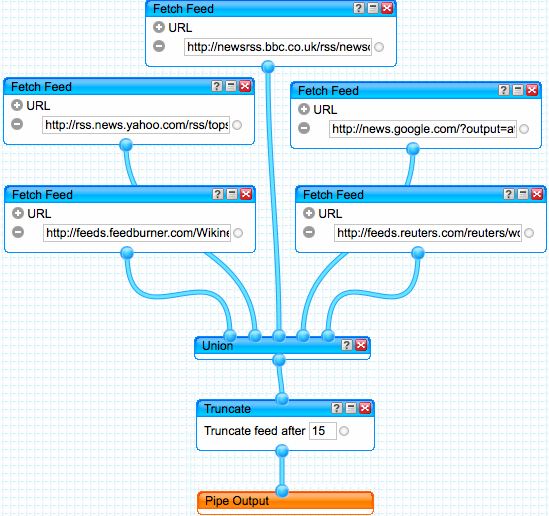
\includegraphics[width=\columnwidth]{yp-1}
\label{fig:ypexample}
\end{figure}


\paragraph{LabVIEW}
\begin{figure}
\caption{Example of a G program from the LabVIEW manual}
\centering
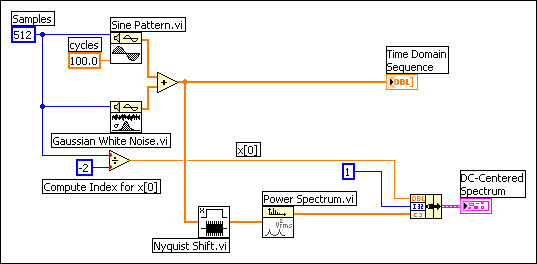
\includegraphics[width=\columnwidth]{labview-1}
\label{fig:labviewexample}
\end{figure}

LabVIEW is a proprietary, visual hardware system design environment which features the visual programming language ``G'' as one of its primary features.
An example of a G program can be found in Figure \ref{fig:labviewexample}.
G is a dataflow language which means a program is represented as a directed graph where data ``flows'' between nodes through their edges.
As such the two most important primitives in G are the edges called \textit{wires} and nodes called \textit{virtual instruments}.
VI's are very similar to functions, because they perform an operation on inputs and provide outputs.
Wires with no source VI are inputs and wires without a destination VI are outputs. 


\section{Smells in end-user programs}
\label{sec:smells}
Research into end-user programming smells has had two approaches, which are not mutually exclusive.
The first approach is to take existing smells for object-oriented programming languages, usually those defined by Fowler, and transform them to be applicable to the end-user environment \cite{Hermans2012inter,Hermans2012intra,Stolee2011,StoleeTSE2013}.
The second approach is to define smells tailored to the end-user environment.
This can be done by interviewing experienced end-users to see which smells they perceive \cite{chambers2013smell}, by looking at user reports like forum or newsgroup posts~ \cite{badame2012refactoring,chambers2013smell}, or by analyzing publicly available artifacts \cite{Stolee2011,StoleeTSE2013}.

This section provides an overview of different smells that researchers have found to be applicable to end-user artifacts.


\begin{table}
\caption{OO Code Smells in End-User Programs \label{table:oosmells}}
\begin{tabular} {| l | l | l | l |}
\hline
\textbf{Smell} & \textbf{Spreadsheets} & \textbf{Yahoo!\ Pipes} & \textbf{LabVIEW} \\ \hline

Feature Envy & ~~ \ding{51}\cite{Hermans2012inter} & ~~ \ding{51}*& ~~  \\ 
Long Method & ~~ \ding{51}\cite{Hermans2012intra} & ~~ \ding{51}* & ~~ \ding{51}*\\
Message Chain & ~~ \ding{51} \cite{Hermans2012intra} & ~~ & ~~ \ding{51} \cite{chambers2013smell} \\
Inappropriate Intimacy & ~~ \ding{51} \cite{Hermans2012inter} & ~~ \ding{51}*& ~~  \\ 
Middle Man & ~~ \ding{51} \cite{Hermans2012inter} & ~~ \ding{51} \cite{StoleeTSE2013}  & ~~  \\
Shotgun Surgery & ~~ \ding{51} \cite{Hermans2012inter} & ~~ & ~~ \\ 
Many Parameters & ~~ \ding{51} \cite{Hermans2012intra} & ~~  \ding{51} \cite{StoleeTSE2013}  & ~~  \ding{51} \cite{chambers2013smell} \\ 
Duplicate Code & ~~ \ding{51} \cite{Hermans2012intra} & ~~ \ding{51} \cite{StoleeTSE2013}  & ~~  \ding{51} \cite{chambers2013smell}\\
Lazy Class & ~~ & ~~ \ding{51} \cite{StoleeTSE2013} & ~~ \ding{51}* \\ 
Dead Code & ~~ \ding{55} & ~~ \ding{51} \cite{StoleeTSE2013} & ~~ \ding{51} \cite{chambers2013smell} \\ 
Unused Field & ~~ \ding{55} & ~~ \ding{51} \cite{StoleeTSE2013} &\\ 

\hline
\multicolumn{4}{c}{} \\ 
\multicolumn{4}{l}{Key:} \\ 
\multicolumn{4}{l}{\ding{55} : Not applicable}\\
\multicolumn{4}{l}{\ding{51} : Applicable, supported in prior work}\\
\multicolumn{4}{l}{\ding{51}* : Likely applicable, future opportunity}\\
\end{tabular}
\end{table}




\subsection{OO Smells in End-User Programs}
 We summarize the OO smells present in the three end-user languages, Microsoft Excel, Yahoo!\ Pipes, and LabVIEW, in Table~\ref{table:oosmells}. Some smells are applicable to the domains but have not yet been studied (\ding{51}*); we discuss these future opportunities in Section~\ref{sec:discussion}. 
 
 Overall, we observe a lot of overlap in the code smells studied. For example, the \emph{Duplicate Code} and \emph{Many Parameters} smells have been studied in all three languages. Other smells, like \emph{Shotgun Surgery}, has only been studied for Excel. \todo{Due to XYZ reason, this smell is not applicable to the other languages}
 
 \subsubsection{Excel}
Hermans et al. \cite{Hermans2012inter} \cite{Hermans2012intra} analogize a workbook to a program, a worksheet to a class inside that program and a cell to a method.
Working from this analogy, the classic Fowler smells can be divided into class and method smells.
The class smells correspond to \textit{inter-sheet} smells and method smells correspond to \textit{intra-sheet} or \textit{intra-cell} smells.

Hermans et al. \cite{Hermans2012inter} define four inter-worksheet smells and define and evaluate threshold for them based on the EUSES spreadsheet corpus \cite{fisher2005euses}.
Fowler's class smells are translated into spreadsheets using the above analogy. 
For example the \textit{Feature Envy} smell indicates that a class uses members of another class more than it uses the members of its own class.
Similarly a cell can use cells of other worksheets more than it uses those of its own sheet, and thus that cell could better be placed in the other sheet.

In \cite{Hermans2012intra}, Hermans et al. define five intra-worksheet or formula smells and again define and evaluate thresholds for them based on the EUSES corpus.
Several method-level smells translate well into cell-level smells, supporting the validity of the above analogy.
\textit{Multiple Calculations} is similar to the \textit{Long method} code smell.
Like a method with many lines or operations can be hard to understand or change, a cell that has a long formula can have the same problem.
Another interesting smell is the \textit{Long Calculation Chain}, which happens because referenced formulas can reference other formulas ad infinitum.
This is very similar to Fowler's \textit{Message Chain} smell.

%Cunha et. al \cite{cunha2012towards} claim to define code smells for spreadsheet, but they take a different approach and  consider the data contained in a spreadsheet.
%However, it is doubtful if these smells qualify as code smells because they are mostly related to user input and not program logic.
%This also causes them to not have an equivalent in general purpose programming languages.
%We refer to related work section \ref{subsec:related_datasmells}.
%




\subsubsection{Yahoo!\ Pipes}
Stolee et al.~\cite{Stolee2011, StoleeTSE2013} treat a Yahoo!\ Pipes mashup as a program and each module as a method.  The most common smell, appearing in nearly one-third of the pipes studied, was \emph{Duplicate Strings}, an instance of Fowler's \emph{Duplicate Code} smell. 
Another common smell, \emph{Duplicate Modules}, impacted nearly one-quarter of the pipes studied. Again, this is an instance of the \emph{Duplicate Code} smell, but at a higher level of abstraction. 

The \emph{Noisy Module} smell impacted 28\% of the pipes studied, and it maps to Fowler's \emph{Unused Field} smell. Here, we found empty or duplicate fields in the pipes, akin to parameters in a method. 

\subsubsection{LabVIEW}

We mapped the following OO smells to the ones defined in prior work\cite{chambers2013smell}: message chain is Multiple Nested Loops , many parameters is Too Many Variables, duplicate code is Redundant operations, and dead code is Unconnected Front Panel
elements. 
\todo{discuss this}

\subsection{Domain-Specific Smells}
The end-user programming environments offer many opportunities to define smells based on user behavior or unique elements of the domain. For example, access to large repositories of programs can lead to smells that deviate from best practices in programming. Systems designed in LabVIEW do not always perform well, leading to the identification of performance smells~\cite{chambers2013smell}. 

\subsubsection{Excel}

\todo{David - Empty cel smell (Cunha)}
\todo{David - Inconsistent formula (as detected by Excel already)}
\todo{David - Add domain-specific smells to table if there's enough}

\subsubsection{Yahoo!\ Pipes}
%Talk about smells unique to the domain
By exploring a large subset of the Yahoo!\ Pipes repository, Stolee et al. identified two smells based on the presence of broken data sources and the use of deprecated modules~\cite{StoleeTSE2013}. These are based on the presence of unsupported, or deprecated, modules, and trying to access an RSS feed that either does not exist or requires special permission. 

%Talk about deriving smells from the community
The presence of a large, publicly available repositories of code opens an opportunity to identify common programming practices, and deviations from those practices as smells. This approach was used to define smells based on community standards for the Yahoo!\ Pipes domain. 



\subsubsection{LabVIEW}

\todo{David - Move parts of this to III.A.3}

The G programs created in LabVIEW do not always perform well, which has motivated Chambers and Scaffidi \cite{chambers2013smell} to define smells in G and implement heuristics to identify these smells, where they particularly focus on smells that can indicate performance problems.

The thirteen smells identified roughly fall into three categories.
The first three are smells specific to the environment, for example the ``\textit{Sequence instead of State machine}'' smell which is a smell because state machines can be much better optimized by the G compiler.

The second and third categories are more broadly applicable, with the second category of two smells being smells you could find a any program that uses concurrency.
One can easily see how ``\textit{Non-reentrant VI}'' is a smell in a language that heavily relies on concurrency and parallelization since such a VI will require blocking and thus possibly slows down the program, similar to how a non-reentrant function could be a problem in a concurrent program written in a general purpose language.

The third and largest category with eight smells are those that are applicable to general purpose languages.
``\textit{Multiple Nested Loops}'' is a smell in almost any language that supports loops, and ``\textit{Build Array inside Loop}'' would be similar to allocating multiple small segments of memory with C's \texttt{malloc} inside a loop with potentially equally bad performance implications.

\subsection{Future Opportunities for Smell Detection}
There are several OO code smells in Table~\ref{fig:ypexample} that apply to all three domains, such as \emph{Duplicate Code}. However, there are other smells that could apply to additional domains, but have not been studied in prior work. Here, we discuss the potential of generalizing smell definitions to additional domains. 

\subsubsection{Excel} \todo{Felienne}
\subsubsection{Yahoo!\ Pipes}
Many of the smells studied in Excel and LabVIEW could apply to Yahoo!\ Pipes, and in particular, \emph{Feature Envy} and \emph{Inappropriate Intimacy}. 
%uses methods of another class excessively - envy
The feature envy smell could also apply when introducing abstraction to Yahoo!\ Pipes programs. For example, if a pipe has several instances of the same subpipe module, this could be related to excessive use of another class and be smelly. 

%depends on implementation of another class too much - intimacy
When a program uses too much abstraction relative to the size of the pipe, for example, if it is composed of only a subpipe and output module, a pipe could suffer from inappropriate intimacy by depending too much on the implementation of the other class. In fact, this smell matters to end-user programmers.  In an empirical evaluation, programmers often preferred pipes without subpipe modules because they were easier to understand~\cite{StoleeTSE2013}. 



\subsubsection{LabVIEW} \todo{David}

\begin{table}
\caption{OO Code Refactoring in End-User Programs \label{table:ooref}}
\begin{tabular} {| l | c | c | c |}
\hline
\textbf{Refactoring} & \textbf{Spreadsheets} & \textbf{Yahoo!\ Pipes} & \textbf{LabVIEW} \\ \hline
Remove Parameter & ~~ \ding{51} \cite{Hermans2012intraExt} & ~~ \ding{51} \cite{StoleeTSE2013}  & ~~ \ding{51}*\\ 
Extract Method & ~~ \ding{51} \cite{Hermans2012intraExt,badame2012refactoring} & ~~ \ding{51}* & ~~ \ding{51}* \\
Inline Method & ~~ \ding{51} \cite{Hermans2012intraExt} & ~~ \ding{51} \cite{StoleeTSE2013} & ~~ \ding{51}* \\
Form Template Method & ~~ & ~~ \ding{51} \cite{StoleeTSE2013}  & ~~ \\ 
Pull Up Method & ~~ & ~~ \ding{51} \cite{StoleeTSE2013}  & ~~ \\ 
Substitute Algorithm & ~~ \ding{51}* & ~~ \ding{51} \cite{StoleeTSE2013}  & ~~ \ding{51}*\\ 
Library Migration~\cite{Balaban:2005:RSC:1103845.1094832} & ~~ \ding{51}* & ~~  \ding{51} \cite{StoleeTSE2013}  & ~~ \ding{51}* \\ 
Define named constant & ~~ \ding{51} \cite{badame2012refactoring} & ~~ & ~~ \\

%Many Parameters & \ding{51} \cite{Hermans2012intra} &  \ding{51} \cite{StoleeTSE2013}  &  \ding{51} \cite{chambers2013smell} \\ 




\hline
\multicolumn{4}{c}{} \\ 
\multicolumn{4}{l}{Key:} \\ 
\multicolumn{4}{l}{\ding{55} : Not applicable}\\
\multicolumn{4}{l}{\ding{51} : Supported in prior work}\\
\multicolumn{4}{l}{\ding{51}* : Likely applicable, future opportunity}\\
\end{tabular}
\end{table}


\section{Refactoring end-user programs}
\label{sec:refactoring}

A way to solve smells is by refactoring, changing the composition of an artifact so that it no longer contains the smell without changing its behavior or output.
Now that we have examined smells, we can continue to the refactoring of end-user programs.

As with the smells, many refactorings are inspired by the OO domain, while others are specific to the end-user domain. Note that prior work in LabVIEW does not define refactorings, creating a clear opportunity for future work. 

\subsection{OO Refactorings}

\subsubsection{Excel}
\todo{David - Divide into subsections like section III}
The first work on spreadsheet refactoring was done by Badame and Dig \cite{badame2012refactoring}.
They define six refactorings applicable to spreadsheets, although the corresponding smells are only implied and not explicitly defined and implement these in an Excel plugin called \textit{REFbook}.
Three of these have to do with preventing errors, like \textit{Guard Call} which places an \texttt{IF} around an expression which can result in an error such as a division by potentially zero.
The other two directly correspond to known smells.
\textit{Extract Row or Column} or more generally \textit{Extract Subformula} is a refactoring with which part of a formula is extracted to a new cell.
This solves the \textit{Multiple operations} smell, which is analogous to the \textit{Long Method} \cite{Hermans2012intra} smell.
A similar operation is the \textit{Extract Literal} refactoring, in which a literal value is extracted formulas into a different cell.
This can solve the \textit{Magic Number} smell.
The last one, \textit{Replace Akward Formula} is very specific and transforms multiple additions into a single \texttt{SUM} operation.

Hermans and Dig \cite{hermans2014bumblebee} take a more generic approach and provide a way to transform spreadsheet formulas to other spreadsheet formulas, in a way that is very similar to how a regular expression or patterns works in some modern programming languages.
They implement this in an Excel plugin called BumbleBee.
To define a transformation rule one defines a formula to match and a formula to replace it with. While every Excel formula can be provided, the power comes from, to use the regular expression terminology, ``capturing groups'' which can bind to a subformula, cell or range. For example, the transformation rule
\[F_1/F_2 \leftrightarrow IF(F_2<>0,F_1/F_2,''undefined'')\]
 implements the \textit{Guard Call} \cite{badame2012refactoring} refactoring by transforming a formula into one which prevents division by zero.
 In this example $F$ can capture (bind to) any valid Excel Formula.
 With this approach it is possible to create a rule for all refactorings defined by Badame and Dig \cite{badame2012refactoring}, but also all refactorings as long as they do not require more intricate capturing groups.
 
\subsubsection{Yahoo!\ Pipes}
The refactorings studied in Yahoo!\ Pipes were target the code smells with the goal of making pipes smaller, less complex, more maintainable, and easier to understand~\cite{StoleeTSE2013}. Some of the refactorings translated easily from the OO domain. For example, removing dead code was as simple as \emph{removing non-contributing modules} or removing fields in \emph{clean up module}~\cite{StoleeTSE2013}. The \emph{Pull up method} refactoring involved extracting a connected set of modules into into a subpipe. Once the subpipe was created, all  parts of the program with the same pattern of connected modules were replaced with the subpipe module. 


\subsection{Domain-Specific Refactorings}

\subsubsection{Excel}

\subsubsection{Yahoo!\ Pipes}
Opportunities for domain-specific refactorings stem from the domain-specific code smells. 
For example, based on the smell of \emph{non-conforming module orderings} where a programming syntax was different than the community standard, the refactoring, \emph{normalize order of operations} was introduced. This refactoring was shown to preferable to end-user programers for improving the understandability of the program~\cite{StoleeTSE2013}. 

\subsection{Future Opportunities for Refactoring}
\subsubsection{Excel}
\subsubsection{Yahoo!\ Pipes}
\todo{Katie}

\subsubsection{LabVIEW}
\todo{David - Divide into subsections like section III}
Chambers and Scaffidi \cite{chambers2013smell} do not provide support for automatic refactorings in their tool, instead relying on the users to know how to fix the indicated smell themselves.
However, the LabVIEW programming language G is a visual dataflow language.
Sui et. al \cite{sui2008automated} have done some work on refactoring visual dataflow languages and defined some refactorings which are applicable to G.
Most notable is the \textit{Extract sub graph into Node} refactoring which is similar to the \textit{Extract Method} refactoring and moves part of a graph into a separate node which is then included in the original graph.
In LabVIEW this could be named \textit{Extract Virtual Instrument}.
However, Sui et. al did not implement their proposed refactorings in an end-user programming environment.







\section{Related Work}
\label{sec:related_work}

\subsection{``Data smells''}
\label{subsec:related_datasmells}

In end-user programming environments user input and logic are often more closely linked than they are in general purpose programming languages.
As such analyzing the input data as opposed to the logic can also be used to detect problems.

Cunha et. al \cite{cunha2012towards} claim to define code smells for spreadsheet, but for most of their smells they look at different types of anomalies in the data of a spreadsheet and define these as smells.
As such ``Data Smell'' is a more appropriate name.
Examples of this are \textit{Standard Deviation} which occur if one assumes a normal distribution for a column in numeric values and the column contains values which fall outside two standard deviations.
They implement detection for their smells in a stand-alone tool called SmellSheet Detective which can analyze spreadsheets from the online office environment Google Docs.

In more recent work Barowy et. Al \cite{barowy2014checkcell} take a very similar but more formalized and thorough approach which they label ``Data Debugging''.
They developed an Excel plugin called CheckCell which uses statistical analysis to find values with an unusually high impact on the calculated results in a spreadsheet.
Such values are likely either very important or erroneous.
While ``Data Debugging'' is a valid term, we think the term ``Data Smell'' is more valid because it shows the similarity to code smells and its similar potential such as locating weak points in the artifact and possibility for refactoring.

\subsection{Testing end user-programs}

\todo{expand}

Refactoring is linked to testing because refactoring an artifact is made safer and easier by the existence of a good test suite in said artifact.

\todo{Mention expector}

\section{Discussion}
\label{sec:discussion}

Based on the research and results for smell detection and refactoring in end-user programming domains, there are many directions for future work in the domains studied, other end-user domains, and in professional languages. 

Note that the authors of this work have pioneered smell detection and refactoring research in spreadsheets and Yahoo!\ Pipes, but are not involved with LabVIEW. Thus, the opportunities for future work in this area may not be complete.  \todo{Is this the best place for the disclaimer?}

\todo{Katie asked Chris for a bit of feedback - waiting on response}



\subsection{Future Opportunities in the Domains Studied}
%YP opportunities
In a qualitative analysis of the end-user preferences for Yahoo!\ Pipes programs, the participant responses showed preference toward programs with familiar elements~\cite{Stolee2015}. This opens an opportunity and perhaps a need to define code smells and refactorings based on end-user experience. 

\subsection{Future Opportunities in Other EUP Domains}
\todo{education (kodu, scratch, alice), mathematics (matlab, mathematica), ...}

\subsection{Future Opportunities in Professional Languages}
In end-user programming languages, it has been shown that code smells impact the understandability of
source code~\cite{StoleeTSE2013}. Additionally, being presented with code smells can motivate end-user programmers to improve their code~\cite{chambers2013smell}. 
\todo{Another lesson from spreadsheets?}
These lessons could extend to other programming languages outside of the end-user programming domains. There has been successful in using automating smell detection, for example, during agile development (e.g.,~\cite{Schumacher:2010:BES:1852786.1852797}). Paired with the end-user evidence, a stronger case can be made to integrate automated smell detection in many domains. 

\todo{Other data flow languages could benefit from \emph{normalize order of operations} to improve understandability (as it does with YP). }

\section{Concluding Remarks}
\label{sec:conclusions}

\newpage
\balance

% Work that wasn't directly referenced but should still appear in the literature list


\bibliographystyle{IEEEtran}
\bibliography{literaturelist}

\end{document}


